\documentclass[a4paper,11pt]{article}
\title{The application of noisy-channel coding techniques to synthetic DNA barcoding}
\author{\begin{tabular}{rl}
                Name:& Izaak van Dongen\\
           EP Mentor:& Nicolle Mcnaughton\\
               Tutor:& Paul Ingham\\
        Candidate No:&  6659\\
        \end{tabular}
        }

% so the title can be accessed by fancyhdr (and is automatically correctly
% spelled etc)
\makeatletter
\let\thetitle\@title
\makeatother

% fonts
\usepackage[p,osf]{cochineal}
\usepackage[scale=.95,type1]{cabin}
\usepackage[cochineal,bigdelims,cmintegrals,vvarbb]{newtxmath}
% fixed width font with 80 chars per listing line
\usepackage[scaled=.94]{newtxtt}
\usepackage[cal=boondoxo]{mathalfa}

% make the document take up more of the page
\usepackage[margin=1in,headheight=13.6pt]{geometry}

% no paragraph indent
\usepackage[parfill]{parskip}

% custom document header/footer
\usepackage{fancyhdr}
\usepackage{lastpage}

\pagestyle{fancy}
\fancyhf{}
\lhead{\thetitle}
\rhead{Izaak van Dongen}
\rfoot{Page \thepage\ of \pageref{LastPage}}

% pretty table rules and multirow entries
\usepackage{booktabs}
\usepackage{multirow}

% plotting mathematical functions (needs version request)
\usepackage{pgfplots}
\pgfplotsset{compat=1.15}

% \url function and clickable table of contents. no ugly red boxes though
\usepackage[hidelinks]{hyperref}

% maths symbols and other stuff (supersedes the ams* packages)
\usepackage{mathtools}

% For framing definitions
\usepackage[framemethod=tikz]{mdframed}
\usepackage[most]{tcolorbox}

\newtcolorbox{definition}{
freelance,
before=\par\vspace{2\bigskipamount}\noindent,
after=\par\bigskip,
frame code={
  \node[
  anchor=south west,
  inner xsep=8pt,
  xshift=8pt,
  rounded corners=5pt,
  font=\bfseries\color{white},
  fill=gray] at (frame.north west) (tit) {\strut Definition:};
  \draw[
  line width=3pt,
  rounded corners=5pt,gray
  ] (tit.west) -| (frame.south west) -- ([xshift=15pt]frame.south west);
},
interior code={},
top=2pt
}

% for better table of contents stuff, providing the \listof* commands and not
% listing the tables in the table of contents
\usepackage[nottoc,notlof,notlot]{tocbibind}

% more advanced handling of utf8 and fonts or something. apparently good to have
\usepackage[utf8]{inputenc}
\usepackage[T1]{fontenc}

% bibliography management with square braces for citations
\usepackage[square,numbers]{natbib}

% graphics, like eps files and stuff (supersedes graphics)
\usepackage{graphicx}

% used to horizontally align floats
\usepackage{subfig}

% used for figures
\usepackage{float}

% needed for colouring and stuff (xcolor supersedes color)
\usepackage{xcolor}

\definecolor{codegreen}{rgb}{ 0,0.6,0}

% listings of code
\usepackage{minted}
\setminted{breaklines,
           breakbytokenanywhere,
           linenos
}
\usemintedstyle{friendly}
% bigger line numbers
\renewcommand\theFancyVerbLine{\footnotesize\arabic{FancyVerbLine}}

% that can break across pages while being captioned figures
\usepackage{caption}
\newenvironment{longlisting}
{\addvspace{\baselineskip}\captionsetup{type=listing}}
{\addvspace{\baselineskip}}

% allow maths to break across pages
\allowdisplaybreaks

\begin{document}
    \maketitle\thispagestyle{empty} % no page number under title
    \tableofcontents
    \listoflistings
    \listoffigures
    \listoftables

%TODO mention versioning and git
%TODO add some wikipedia citations for bulk/evaluation
%TODO interesting as relatively new field of biology, combined with ancient
%mathematics

%TODO talk about sphere packing
%TODO add mindmap

    \section[Definitions and conventions]{Definitions \footnote{Please note that
    these definitions have been somewhat simplified. It would be impractical and
    outside of the scope of this dissertation to deliver a full briefing of
    the field of computer science.} and conventions}

    My project will involve a lot of programming. Because of the tendency for
    programmers to use field-specific vocabulary/jargon, I have provided the
    following definitions of various words I might use when talking about
    programs I write.

    \begin{definition}
    A \textbf{program} or \textbf{script}, but not to be
    confused with ) is a series of
    instructions that the computer follows in order to complete a task. They are
    normally created and shown in the form of text. Roughly speaking, each line
    of text corresponds to one instruction for the computer to follow. A program
    in this form is written in a programming language.
    \end{definition}

    \begin{definition}
    A program normally also permits \textbf{input}, \textbf{arguments} or
    \textbf{parameters}. These allow a user of the program to feed it some data
    or starting instructions. This is extremely useful as it means that the
    program doesn't just do the same thing each time, but performs its task on
    the data or information requested by the user.
    \end{definition}

    \begin{definition}
    The word \textbf{code} sits kind of annoyingly here. Code may both refer to
    programming instructions or systems of symbols representing data. When
    referring to programs, code is an uncountable noun, eg ``I wrote some
    code''. When referring to symbolic systems, it \textit{is} countable, so you
    might say ``I generated some code\textit{s}, using the code I wrote earlier.
    \end{definition}

    \begin{definition}
    The programs I produce will be CLI-based. That is, they will use a
    \textbf{Command Line Interface}. This means that the user interacts with the
    program solely through text. Most applications nowadays use a graphical
    interface, but a CLI has many benefits, including but not limited to being
    easier to develop, being faster due to less overhead, CLI programs can
    interact with each other more easily as it provides a standard interface,
    and they are more portable. The downside of course is that it required more
    expertise to use.

    An example of how I use the CLI to interact with a program is given in
    Figure \ref{fig:cliusage}.
    \end{definition}

\begin{figure}[H]
\begin{center}
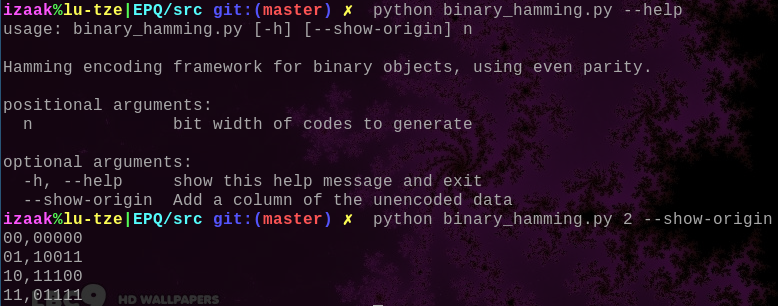
\includegraphics[width=0.8\textwidth]{../images/cli_usage.png}
\end{center}
\caption{Example of a CLI interface}\label{fig:cliusage}
\end{figure}

    \begin{definition}
    A \textbf{programming language} is a defined language that both the computer
    and the programmer understand.  The programming language I'm using for this
    dissertation is Python. To produce some of by graphics, I'm using
    Postscript. On a more meta-level this dissertation itself has been produced
    with \LaTeX, and I have worked on it on a GNU/Linux system, making use of
    the shell language Zsh, and other tools like the language `Make'. None of
    these are particularly important to understanding the outcome or goals of
    this dissertation.
    \end{definition}

    \begin{definition}
    A \textbf{comment} is a section of a program which has been specially marked
    to be ignored by the computer. These are used by humans to add documentation
    or clarification to code, and are written in natural language.  In the two
    languages I'm using, comments are marked by a preceding \% or \#.
    \end{definition}

    \begin{definition}
    A \textbf{docstring} is also text within a program. It is similar to a
    comment, but there are some technical and semantic differences. Most
    importantly, a docstring is intended to describe the function of some unit
    of the code. This might be one function, one class, or of the whole program.
    A docstring is enclosed by three consecutive double quotes:
    \mintinline{python}|"""|. By convention, docstrings are written in the
    imperative mood \cite{PEPDocstrings2014Goodger}.
    \end{definition}

    \begin{definition}
    A \textbf{function} is a part of the code that acts out one specific task.
    These are useful as they can be reused, making code more maintainable (only
    one part must be modified), shorter and easier to test. Functions in Python
    are generally preceded by \mintinline{python}|def
    function_name(parameters):|.  Here, `parameters` defines which inputs the
    function expects. This allows the function to perform the same task on
    different data. All of the code within the function will then be indented
    one level.
    \end{definition}

    \begin{definition}
    One program can reuse a function from another program. To do this, the
    requesting program must \textbf{import} the function from the defining
    program. Most language also have a standard library of useful functions, so
    some imports will be from the language itself, rather than another file
    within this EP.
    \end{definition}

    \begin{definition}
    A \textbf{unit test} is a way to test that a program is functioning
    correctly. It works by running a number of tests against each \textit{unit}
    of code. These units are normally functions. By making sure that each
    function works, we can be reasonably confident in how robust our code is. A
    unit test is itself also a program.
    \end{definition}

    \begin{definition}
    A \textbf{matrix} is a rectangular array of numbers. They are denoted like:
    \begin{math}
    M =
    \begin{pmatrix}
    1 & 2 & 3 \\
    4 & 5 & 5 \\
    \end{pmatrix}
    \end{math}.
    Matrices have \textbf{rows} and \textbf{columns}, which may have certain
    properties desirable for barcodes.
    \end{definition}

    For my EP I have written several programs. Almost all of these are included
    within the dissertation or some other component as code listings.. When
    appropriate, I have added comments and docstrings to these, to explain
    (commentate) their function.

    In the code listings provided, comments should be highlighted
    \mintinline{python}|#like this|, and docstrings
    \mintinline{python}|"""like this"""|. All of this is demonstrated in listing
    \ref{lst:commentexample}.

\begin{longlisting}
\begin{minted}{python}
#!/usr/bin/env python3
#^ This part is a shebang. It tells the computer what language I'm using

"""
This part is a docstring and explains what all of the code does
"""

import pprint
import json

def this_is(some: "code") -> {"th": at}:
    """
    This is another docstring, but in a function, to describe what the function
    does.
    """
    for x in y:
        pprint(json.loads('{"a": 2}'))
        # This part is a comment. It explains what the following line of code
        # does, because it is particularly interesting/complicated.
        does(stuff)

        this is {a: really(long-line(of + code, [that, goes], off(the_edge), resulting in "a little arrow"}

# <- this is a comment pointing out the line numbers
\end{minted}
\caption{Example of a code listing with comments}\label{lst:commentexample}
\end{longlisting}

    \section{Introduction}
    The premise of this project is to investigate the different types of
    error-correcting codes, and how these might be applied to DNA barcoding. DNA
    barcoding is the assignment of `barcodes' to subsequences of synthesised DNA
    for the purposes of identification. This means that in future, when you look
    at that same subsequence, that should let you `ID' the whole DNA sequence.
    However, as we all know, DNA is subject to mutation, so an ideal barcode
    should still be identifiable after some number of mutations. This is where
    error-correcting codes come in.

%TODO maybe some citations
% also
%- crispr/cas9 citations

    The challenge in this comes from the fact that most error-correcting codes
    are designed in base-2 (binary) whereas DNA strings are fundamentally
    base-4 (quaternary). The applicability of this project is that in
    oligonucleotide synthesis, some samples may need to be identified later on
    using a subsection of the sample (a barcode). These could just be linearly
    assigned codes, but this would leave them very susceptible to mutation.

    Here is an example: say that we're given a barcode of length four, to encode
    two different samples. If we worked methodically up from the bottom (using
    the ordering \texttt{ACGT} - orderings will be discussed further later on)
    we might end up with the codes \texttt{AAAA} and \texttt{AAAC}. However,
    either string would only require a single mutation (where we say a mutation
    is the changing of a single base) to become identical to the other one.
    Therefore, in this case, it would clearly be far more optimal to make a
    choice like, for example, \texttt{AAAA} and \texttt{CCCC} (although this
    leaves you with only two different codes).

    We have kind of glossed over how we in this case formally represent DNA and
    mutations, but we will get to that.

    There are also a number of parameters to the problem, and as they change
    the problem becomes increasingly hard:

    \begin{itemize}
    \item What if the barcode size changes?
    \item What if we want more codes than two?
    \item What if we anticipate many mutations?
    \end{itemize}

    All of these will be further explored in this dissertation.

    \section[Applications]{Applications \footnote{This section gives a brief
    overview of possible applications - be aware that this is somewhat
    abbreviated as this topic is not the focus of this dissertation.}}

    You may well have heard of CRISPR/Cas9, depending on which news sources you
    follow. CRISPR stands for ``Clustered Regularly Interspaced Short
    Palindromic Repeats'', which is a family of DNA sequences in bacteria
    \cite{CRISPRDailyMail,CRISPRImmune2010Horvath,WikiCrispr}. Cas9 is a
    specific CRISPR Associated Protein \cite{WikiCas9}. Together, they provide a
    mechanism for the editing of the DNA of an organism
    \cite{CRISPER2016Finneran}, by using a specific kind of virus.  This
    mechanism is shown in figure \ref{fig:crispr}.

\begin{figure}[H]
\begin{center}
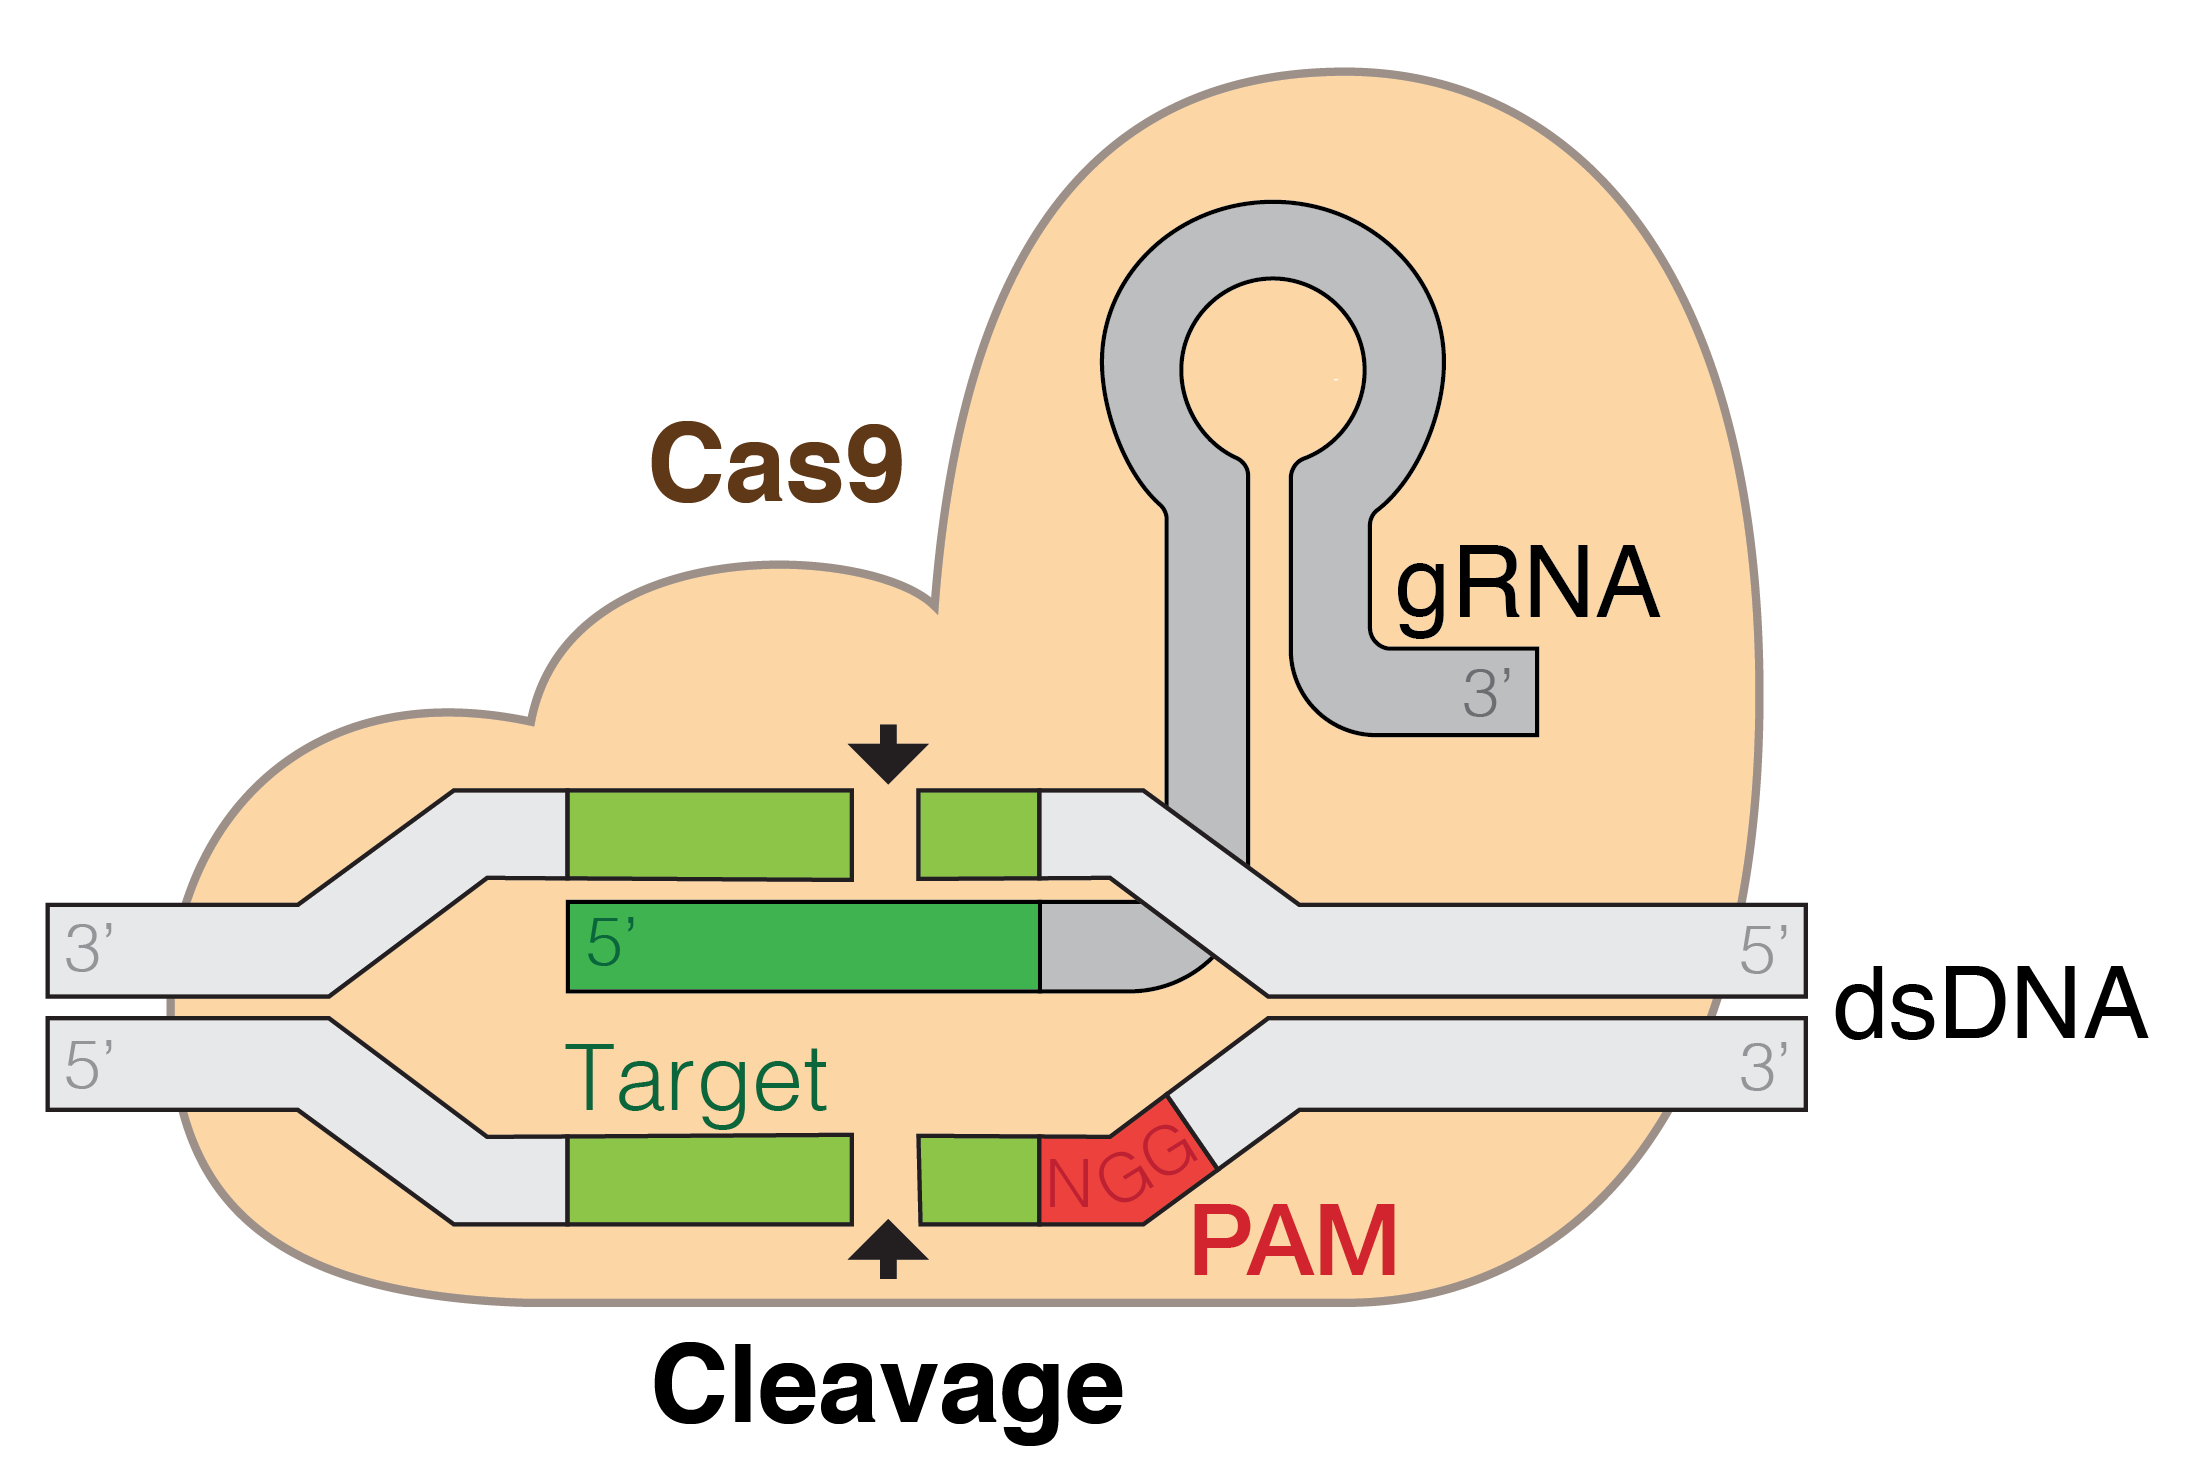
\includegraphics{../images/GRNA-Cas9.png}
\end{center}
\caption{Illustration of CRISPR editing DNA}\label{fig:crispr}
\end{figure}

    This mechanism requires ``guide RNA (gRNA)''. This RNA may sometimes have to
    be synthesised on a large scale, and this is where the barcodes come in. If
    a large ``batch'' of gRNA contains RNA to be used for different experiments,
    this could then be barcoded in order to identify the RNA.

    This is just one example of what could be done - there are many other
    applications \cite{WikiBarcoding}.

    \section{The Hamming distance}

    The Hamming distance is a measure of ``string distance''. String
    distance is a way to define how different two string are.
    Coding-theoretically, this can be used to quantify the amount that a
    string has been changed by transmission (or an oligonucleotide has been
    mutated).

    The Hamming distance between any two equally long strings $S$ and $R$
    is given by the number of characters at identical position that differ.
    For example, if we let $d_H$ denote Hamming distance, the distances
    \begin{align*}
    d_H(S, R) &= 1\\
    d_H(S, T) &= 2\\
    \text{where}\
    S &= \texttt{abcde}\\
    R &= \texttt{abc\textcolor{blue}{f}e}\\
    T &= \texttt{a\textcolor{codegreen}{x}c\textcolor{codegreen}{z}e}
    \end{align*}
    Note that for any $S$, $d(S, S) = 0$. This means that there is no
    ``distance'' from a string to itself.

    In terms of DNA, the Hamming distance can be used to determine the
    number of bases that have mutated.

%TODO citation needed

    \section{Parity codes}

    \subsection{Parity}

    The insertion of ``parity bits'' is a common practice in basic encoding.
    Parity refers to the ``oddness'' or ``evenness'' of some data
    \cite{Parity2008Knuth}.

    Commonly, this is determined by making sure that the sum of the data is $0
    \mod 2$. This is also known as ``even parity'', and means that the total
    number of $1$-bits in the data should be even.  This means that the data is
    known to have been corrupted if its sum is odd.

    The reason that I am using such an elaborate definition with sums and
    moduluses is that I know I want to adapt my codes to base 4, and by using
    such a general definition, this is done quite easily.

% correct this with regard to odd parity

    \subsection{Simple example}

    A simple but inefficient parity encoding scheme is a column/row wise
    encoding \cite{CodeIntro2010Guruswami}. Take the slightly contrived data
    string ``\texttt{0100000101010100}''.  This is very tangentially related to
    DNA - it's the 8-bit ASCII \cite{ASCII1963ASA} representation of the string
    ``AT'', generated by the Python:
    \mintinline{python}|"".join(bin(ord(c))[2:].rjust(8, "0") for c in "AT")|
    \footnote{Sometimes I will include some `meta-code' that was used to
    generate a table or other data. Especially the smaller samples won't be as
    extensively commented as I don't consider these core programs - they are a
    kind of shortcut from writing the table out by hand.}.

    The string is then arranged in a square like so:

    \begin{center}
    \texttt{
    \begin{tabular}{cccc}
        0 & 1 & 0 & 0 \\
        0 & 0 & 0 & 1 \\
        0 & 1 & 0 & 1 \\
        0 & 1 & 0 & 0
    \end{tabular}
    }
    \end{center}

    An extra row and column, including an extra corner piece is appended like
    so:

    \begin{center}
    \texttt{
    \begin{tabular}{c c c c | c}
        0 & 1 & 0 & 0 & 1 \\
        0 & 0 & 0 & 1 & 1 \\
        0 & 1 & 0 & 1 & 0 \\
        0 & 1 & 0 & 0 & 1 \\ \hline
        0 & 1 & 0 & 0 & 1
   \end{tabular}
   }
   \end{center}

   Each of the extra bits documents the parity of its row. Using a scheme like
   this, a single corrupted bit can be detected, and corrected. For example,
   the bit at (3, 4) may have flipped like so:

    \begin{center}
    \texttt{
    \begin{tabular}{c c c c | c}
        0 & 1 & 0 & 0 & 1 \\
        0 & 0 & 0 & 1 & 1 \\
        0 & 1 & 0 & 1 & 0 \\
        0 & 1 & \textcolor{red}{1} & 0 & 1 \\ \hline
        0 & 1 & 0 & 0 & 1
   \end{tabular}
   }
   \end{center}

    Someone wishing to correct this error can check the parity of each column,
    compared with its parity bit. They can do the same for each row. Assuming
    one error has occurred, the point where the incorrect row and column cross
    is to be flipped back. In this case, the third column doesn't add up, and
    the fourth row doesn't add up, leading to the faulty bit. It is worth
    noting that this also works to correct errors in the parity bits, due the
    the extra corner bit. If only the extra corner bit seems to be wrong, it is
    the one that has flipped.

    \subsection{Limitations}

    This particularly scheme is in a sense quite inefficient. At the
    most optimal configuration, it uses on the order of $2\sqrt{n}$ parity bits,
    where $n$ is the number of bits in the message, in order to achieve 1
    correction. This can be proven as follows:

    Assume $n$ to be highly divisible. Let $p$ denote the number of parity
    bits, and $x$ denote the length of a row. We then have,

    \begin{align*}
        p &= \frac{n}{x} + x \\
        \Rightarrow \frac{dp}{dx} &= 1 - \frac{n}{x^2}
                    = 0\ \text{(as $p$ is a minimum)}\\
        \Rightarrow 1 &= \frac{n}{x^2} \\
        \Rightarrow x^2 &= n \\
        \Rightarrow x &= \sqrt{n} \\
        \Rightarrow p &= \frac{n}{\sqrt{n}} + \sqrt{n} = \sqrt{n} + \sqrt{n} \\
                      &= 2\sqrt{n} \\
    \end{align*}

    This is quite a poor asymptotic performance - as the number of data bits
    grows larger, the number of parity bits required grows relatively fast. In
    the next section, I describe a similar code that uses only $\log_2 n$. In
    figure \ref{fig:logsqrtplot} is a quick plot comparing the two functions.

\begin{figure}[H]
\begin{center}
    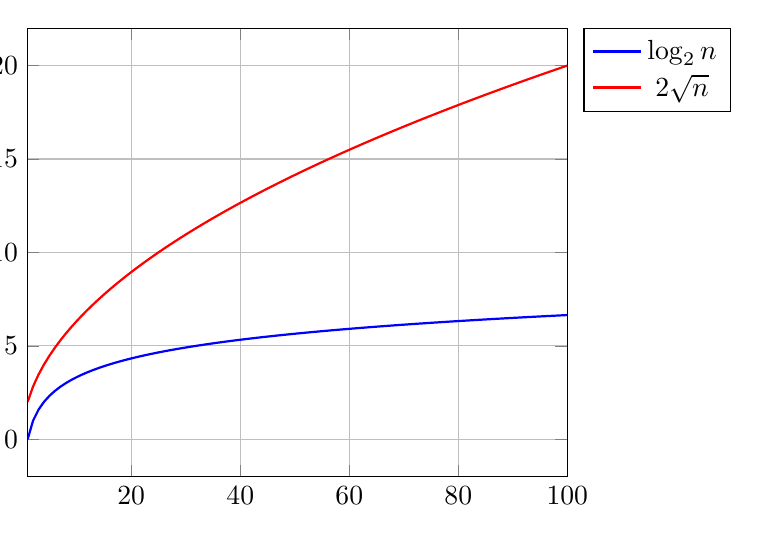
\begin{tikzpicture}[trim axis left]
    \begin{axis}[
      domain=1:100,
      no markers,
      samples=100,
      enlarge x limits=false,
      grid=both,
legend entries={$\log_2 n$,
                $2\sqrt{n}$},
legend pos=outer north east]
    \addplot +[thick] {ln(x)/ln(2)};
    \addplot +[thick] {2 * sqrt(x)};
    \end{axis}
    \end{tikzpicture}
\end{center}
\caption{Asymptotic performance of $\log$ and $\sqrt{}$}\label{fig:logsqrtplot}
\end{figure}

    As you can see, as $n$ increases the relative performance of the row-column
    approach degrades significantly.

    \section{The Hamming code}

    \subsection{Description}

    The Hamming code instead places a parity bit at each index that is a power
    of two, where we number indices starting from 1. Therefore, our previous
    data string gains parity bits in this configuration:
    \texttt{\textcolor{red}{10}0\textcolor{red}{1}100\textcolor{red}{0}0001010\textcolor{red}{0}10100}
    (the 1st, 2nd, 4th, 8th and 16th bits are used for parity).

    The way the parity ``coverage'' works is shown in table
    \ref{tab:hamming-indices}.  I have included indices up to 31. This is
    because that is the longest encodable string with only five parity bits
    (afterwards, we have to add a parity bit at 32). Of course, a shorter code
    word can always also be encoded by just acting as if each index that is out
    of range stores a 0.

\begin{table}[H]
\begin{center}
    \begin{tabular}{crrrrrrrrrrrrrrr}
    \toprule
    Parity index & \multicolumn{15}{c}{Covered indices} \\
    \midrule
    1 & 3 & 5 & 7 & 9 & 11 & 13 & 15 & 17 & 19 & 21 & 23 & 25 & 27 & 29 & 31 \\
    2 & 3 & 6 & 7 & 10 & 11 & 14 & 15 & 18 & 19 & 22 & 23 & 26 & 27 & 30 & 31 \\
    4 & 5 & 6 & 7 & 12 & 13 & 14 & 15 & 20 & 21 & 22 & 23 & 28 & 29 & 30 & 31 \\
    8 & 9 & 10 & 11 & 12 & 13 & 14 & 15 & 24 & 25 & 26 & 27 & 28 & 29 & 30 & 31 \\
    16 & 17 & 18 & 19 & 20 & 21 & 22 & 23 & 24 & 25 & 26 & 27 & 28 & 29 & 30 & 31 \\
    \bottomrule
    \end{tabular}
    \caption{Parity coverage in a Hamming code}\label{tab:hamming-indices}
\end{center}
\end{table}

    These are very deliberately chosen indices. In fact, this table was
    generated by a short code snippet that can be found in listing
    \ref{lst:hamtab}.

    The way that it works is by considering the value of the parity index in
    binary. For example, $4_{10}=100_{2}$. As they are powers of two, they will
    always be of the form `$10*$' (a one followed by 0 or more zeroes).

    The code in listings \ref{lst:hamcol} and \ref{lst:hamps} generates two
    visualisations, which I find helpful. The first is table
    \ref{tab:hamming-binary}, which is similar to table
    \ref{tab:hamming-indices}, but transposed so each column corresponds to a
    parity bit, and each index is written in binary:

\begin{table}[H]
\begin{center}
    \begin{tabular}{l|rrrrr}
    \toprule
    Parity index & \texttt{0000\textcolor{blue}{1}} & \texttt{000\textcolor{blue}{1}0} & \texttt{00\textcolor{blue}{1}00} & \texttt{0\textcolor{blue}{1}000} & \texttt{\textcolor{blue}{1}0000} \\
    \midrule
    \multirow{14}{*}{Coverage}
    & \texttt{0001\textcolor{blue}{1}} & \texttt{000\textcolor{blue}{1}1} & \texttt{00\textcolor{blue}{1}01} & \texttt{0\textcolor{blue}{1}001} & \texttt{\textcolor{blue}{1}0001} \\
    & \texttt{0010\textcolor{blue}{1}} & \texttt{001\textcolor{blue}{1}0} & \texttt{00\textcolor{blue}{1}10} & \texttt{0\textcolor{blue}{1}010} & \texttt{\textcolor{blue}{1}0010} \\
    & \texttt{0011\textcolor{blue}{1}} & \texttt{001\textcolor{blue}{1}1} & \texttt{00\textcolor{blue}{1}11} & \texttt{0\textcolor{blue}{1}011} & \texttt{\textcolor{blue}{1}0011} \\
    & \texttt{0100\textcolor{blue}{1}} & \texttt{010\textcolor{blue}{1}0} & \texttt{01\textcolor{blue}{1}00} & \texttt{0\textcolor{blue}{1}100} & \texttt{\textcolor{blue}{1}0100} \\
    & \texttt{0101\textcolor{blue}{1}} & \texttt{010\textcolor{blue}{1}1} & \texttt{01\textcolor{blue}{1}01} & \texttt{0\textcolor{blue}{1}101} & \texttt{\textcolor{blue}{1}0101} \\
    & \texttt{0110\textcolor{blue}{1}} & \texttt{011\textcolor{blue}{1}0} & \texttt{01\textcolor{blue}{1}10} & \texttt{0\textcolor{blue}{1}110} & \texttt{\textcolor{blue}{1}0110} \\
    & \texttt{0111\textcolor{blue}{1}} & \texttt{011\textcolor{blue}{1}1} & \texttt{01\textcolor{blue}{1}11} & \texttt{0\textcolor{blue}{1}111} & \texttt{\textcolor{blue}{1}0111} \\
    & \texttt{1000\textcolor{blue}{1}} & \texttt{100\textcolor{blue}{1}0} & \texttt{10\textcolor{blue}{1}00} & \texttt{1\textcolor{blue}{1}000} & \texttt{\textcolor{blue}{1}1000} \\
    & \texttt{1001\textcolor{blue}{1}} & \texttt{100\textcolor{blue}{1}1} & \texttt{10\textcolor{blue}{1}01} & \texttt{1\textcolor{blue}{1}001} & \texttt{\textcolor{blue}{1}1001} \\
    & \texttt{1010\textcolor{blue}{1}} & \texttt{101\textcolor{blue}{1}0} & \texttt{10\textcolor{blue}{1}10} & \texttt{1\textcolor{blue}{1}010} & \texttt{\textcolor{blue}{1}1010} \\
    & \texttt{1011\textcolor{blue}{1}} & \texttt{101\textcolor{blue}{1}1} & \texttt{10\textcolor{blue}{1}11} & \texttt{1\textcolor{blue}{1}011} & \texttt{\textcolor{blue}{1}1011} \\
    & \texttt{1100\textcolor{blue}{1}} & \texttt{110\textcolor{blue}{1}0} & \texttt{11\textcolor{blue}{1}00} & \texttt{1\textcolor{blue}{1}100} & \texttt{\textcolor{blue}{1}1100} \\
    & \texttt{1101\textcolor{blue}{1}} & \texttt{110\textcolor{blue}{1}1} & \texttt{11\textcolor{blue}{1}01} & \texttt{1\textcolor{blue}{1}101} & \texttt{\textcolor{blue}{1}1101} \\
    & \texttt{1110\textcolor{blue}{1}} & \texttt{111\textcolor{blue}{1}0} & \texttt{11\textcolor{blue}{1}10} & \texttt{1\textcolor{blue}{1}110} & \texttt{\textcolor{blue}{1}1110} \\
    & \texttt{1111\textcolor{blue}{1}} & \texttt{111\textcolor{blue}{1}1} & \texttt{11\textcolor{blue}{1}11} & \texttt{1\textcolor{blue}{1}111} & \texttt{\textcolor{blue}{1}1111} \\
    \bottomrule
    \end{tabular}
    \caption{Indices covered by each parity bit shown in binary}\label{tab:hamming-binary}
\end{center}
\end{table}

    The second is shown in figure \ref{fig:hamming}. It represents each covered
    bit as a filled in square, and each non-covered bit as an empty square, so
    the whole codeword is shown in every row.

\begin{figure}[H]
\begin{center}
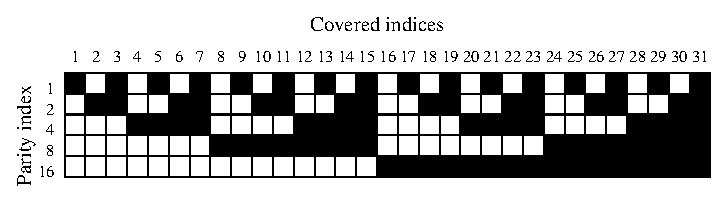
\includegraphics{../psfiles/hamming_visualisation.eps}
\end{center}
\caption{Index coverage of Hamming parity bits}\label{fig:hamming}
\end{figure}

    Now, when decoding a Hamming-encoded message, you check each parity bit for
    errors, as normal. You then add the index of each parity bit that shows an
    error to find the index of the corrupted bit. This bit can then be flipped.
    This can only correct one error, but it is a very effective way to do so -
    in fact, if you only want to correct one error, the Hamming code is optimal
    \cite{Codes1950Hamming}.

    Of course, the Hamming code is not explicitly a way to generate barcodes -
    it is rather an encoding. However, error-correcting encodings can simply be
    applied to all possible strings to generate a set of barcodes. As we are
    using binary for now, you could generate the code corresponding to each of
    the 16 binary strings from \texttt{0000} to \texttt{1111}. This gives you 16
    barcodes of length 7 each, which can be decoded to retrieve the unique
    identifier from 0 to 15 that was associated with the DNA.

    Listing \ref{lst:hammingbin} shows the program that implements a binary
    Hamming encoding. It is tested by the code in listing
    \ref{lst:testhammingbin}.

    \subsection{Implementation}

\begin{longlisting}
\inputminted{python}{../src/encode_hamming.py}
\caption{Binary Hamming code in Python}\label{lst:hammingbin}
\end{longlisting}

    \subsection{Adaption}

    Unfortunately, this all produces binary codes, as this is more of a
    `fundamental' base in the world of computers.. As is, this is of no use
    because DNA strings are fundamentally base-4.

    \subsubsection{Na\"ive approach}

    We are quite fortunate in that 4 is a power of 2. This means that
    we can directly translate a base-4 string to binary, in the case of DNA
    perhaps by mapping \texttt{ACGT} to \texttt{00 01 10 11}.

    This specific ordering is quite useful as each base pair A-T and C-G is a
    set of additive inverses mod 4, or ``number bonds to 4''.

    In any case, by writing a short program to perform this mapping, it is quite
    trivially done.

    \subsubsection{Clever approach}

    It is also possible to directly translate

    \section{The Hadamard code}

    \subsection{Description}

    The Hadamard code is based on Hadamard matrices. A Hadamard matrix is a
    matrix such that each pair of rows represent a pair of orthogonal vectors
    \cite{HadamardMatrices1978HedayatWallis}.
    Practically, this means that each row has a Hamming distance of at least
    half of its length from each other row. This is a much stronger encoding
    than the Hamming code, so may be much more resistant to mutations. However,
    as a natural side effect of this, Hadamard codes are longer and more sparse.

    A basic generation scheme for a sequence of Hadamard matrices $H_{2^n}$ is given
    by Sylvester's construction \cite{OrthogonalMatrix1867Sylvester}:

    \begin{align*}
    H_1 &=
    \begin{pmatrix}
    1\\
    \end{pmatrix} \\
    H_2 &=
    \begin{pmatrix}
    1 &  1 \\
    1 & -1 \\
    \end{pmatrix} \\
    H_{2^{n + 1}} &=
    \begin{pmatrix}
    H_{2^n} &  H_{2^n} \\
    H_{2^n} & -H_{2^n} \\
    \end{pmatrix} =
    H_2 \otimes H_{2^n}
    \end{align*}

    ie the next matrix is

    \begin{math}
    H_4 =
    \begin{pmatrix}
    \begin{pmatrix}
    1 &  1 \\
    1 & -1 \\
    \end{pmatrix} &
    \begin{pmatrix}
    1 &  1 \\
    1 & -1 \\
    \end{pmatrix} \\
    \begin{pmatrix}
    1 &  1 \\
    1 & -1 \\
    \end{pmatrix} &
    -\begin{pmatrix}
    1 &  1 \\
    1 & -1 \\
    \end{pmatrix} \\
    \end{pmatrix} =
    \begin{pmatrix}
    1 &  1 &  1 &  1 \\
    1 & - 1 &  1 & - 1 \\
    1 &  1 & - 1 & - 1 \\
    1 & - 1 & - 1 &  1 \\
    \end{pmatrix}
    \end{math}

    Note this construction's use of the ($-$) operator, together with the set
    $\{1,-1\}$ as it's ``alphabet''. This is necessary for the satisfication of
    the ``orthogonality'' definition of Hadamard matrices, but, in fact, we need
    only a slightly weaker property, which is half of the items being different.
    I have therefore slightly modified this construction to use the Boolean
    alphabet $\{0,1\}$, and use the Boolean logical not ($\lnot$)
    \cite{BooleRecords1956Kneale}. This is more suited to this application of
    these codes, as 0 and 1 are the fundamental numbers that computers work with
    (known as ``bits''), so this makes the implementation more natural and
    elegant, as most programming languages have built in support for Boolean
    logic.

    The code implementing Sylvester's construction can be found in listing
    \ref{lst:hadgen}.

    A visualistion of the Hadamard matrix is provided by the Python script in
    listing \ref{lst:hadpy}. It displays the matrix as a grid, where each `1' is
    filled in, as in figure \ref{fig:hadvis}.

\begin{figure}[H]
\begin{center}
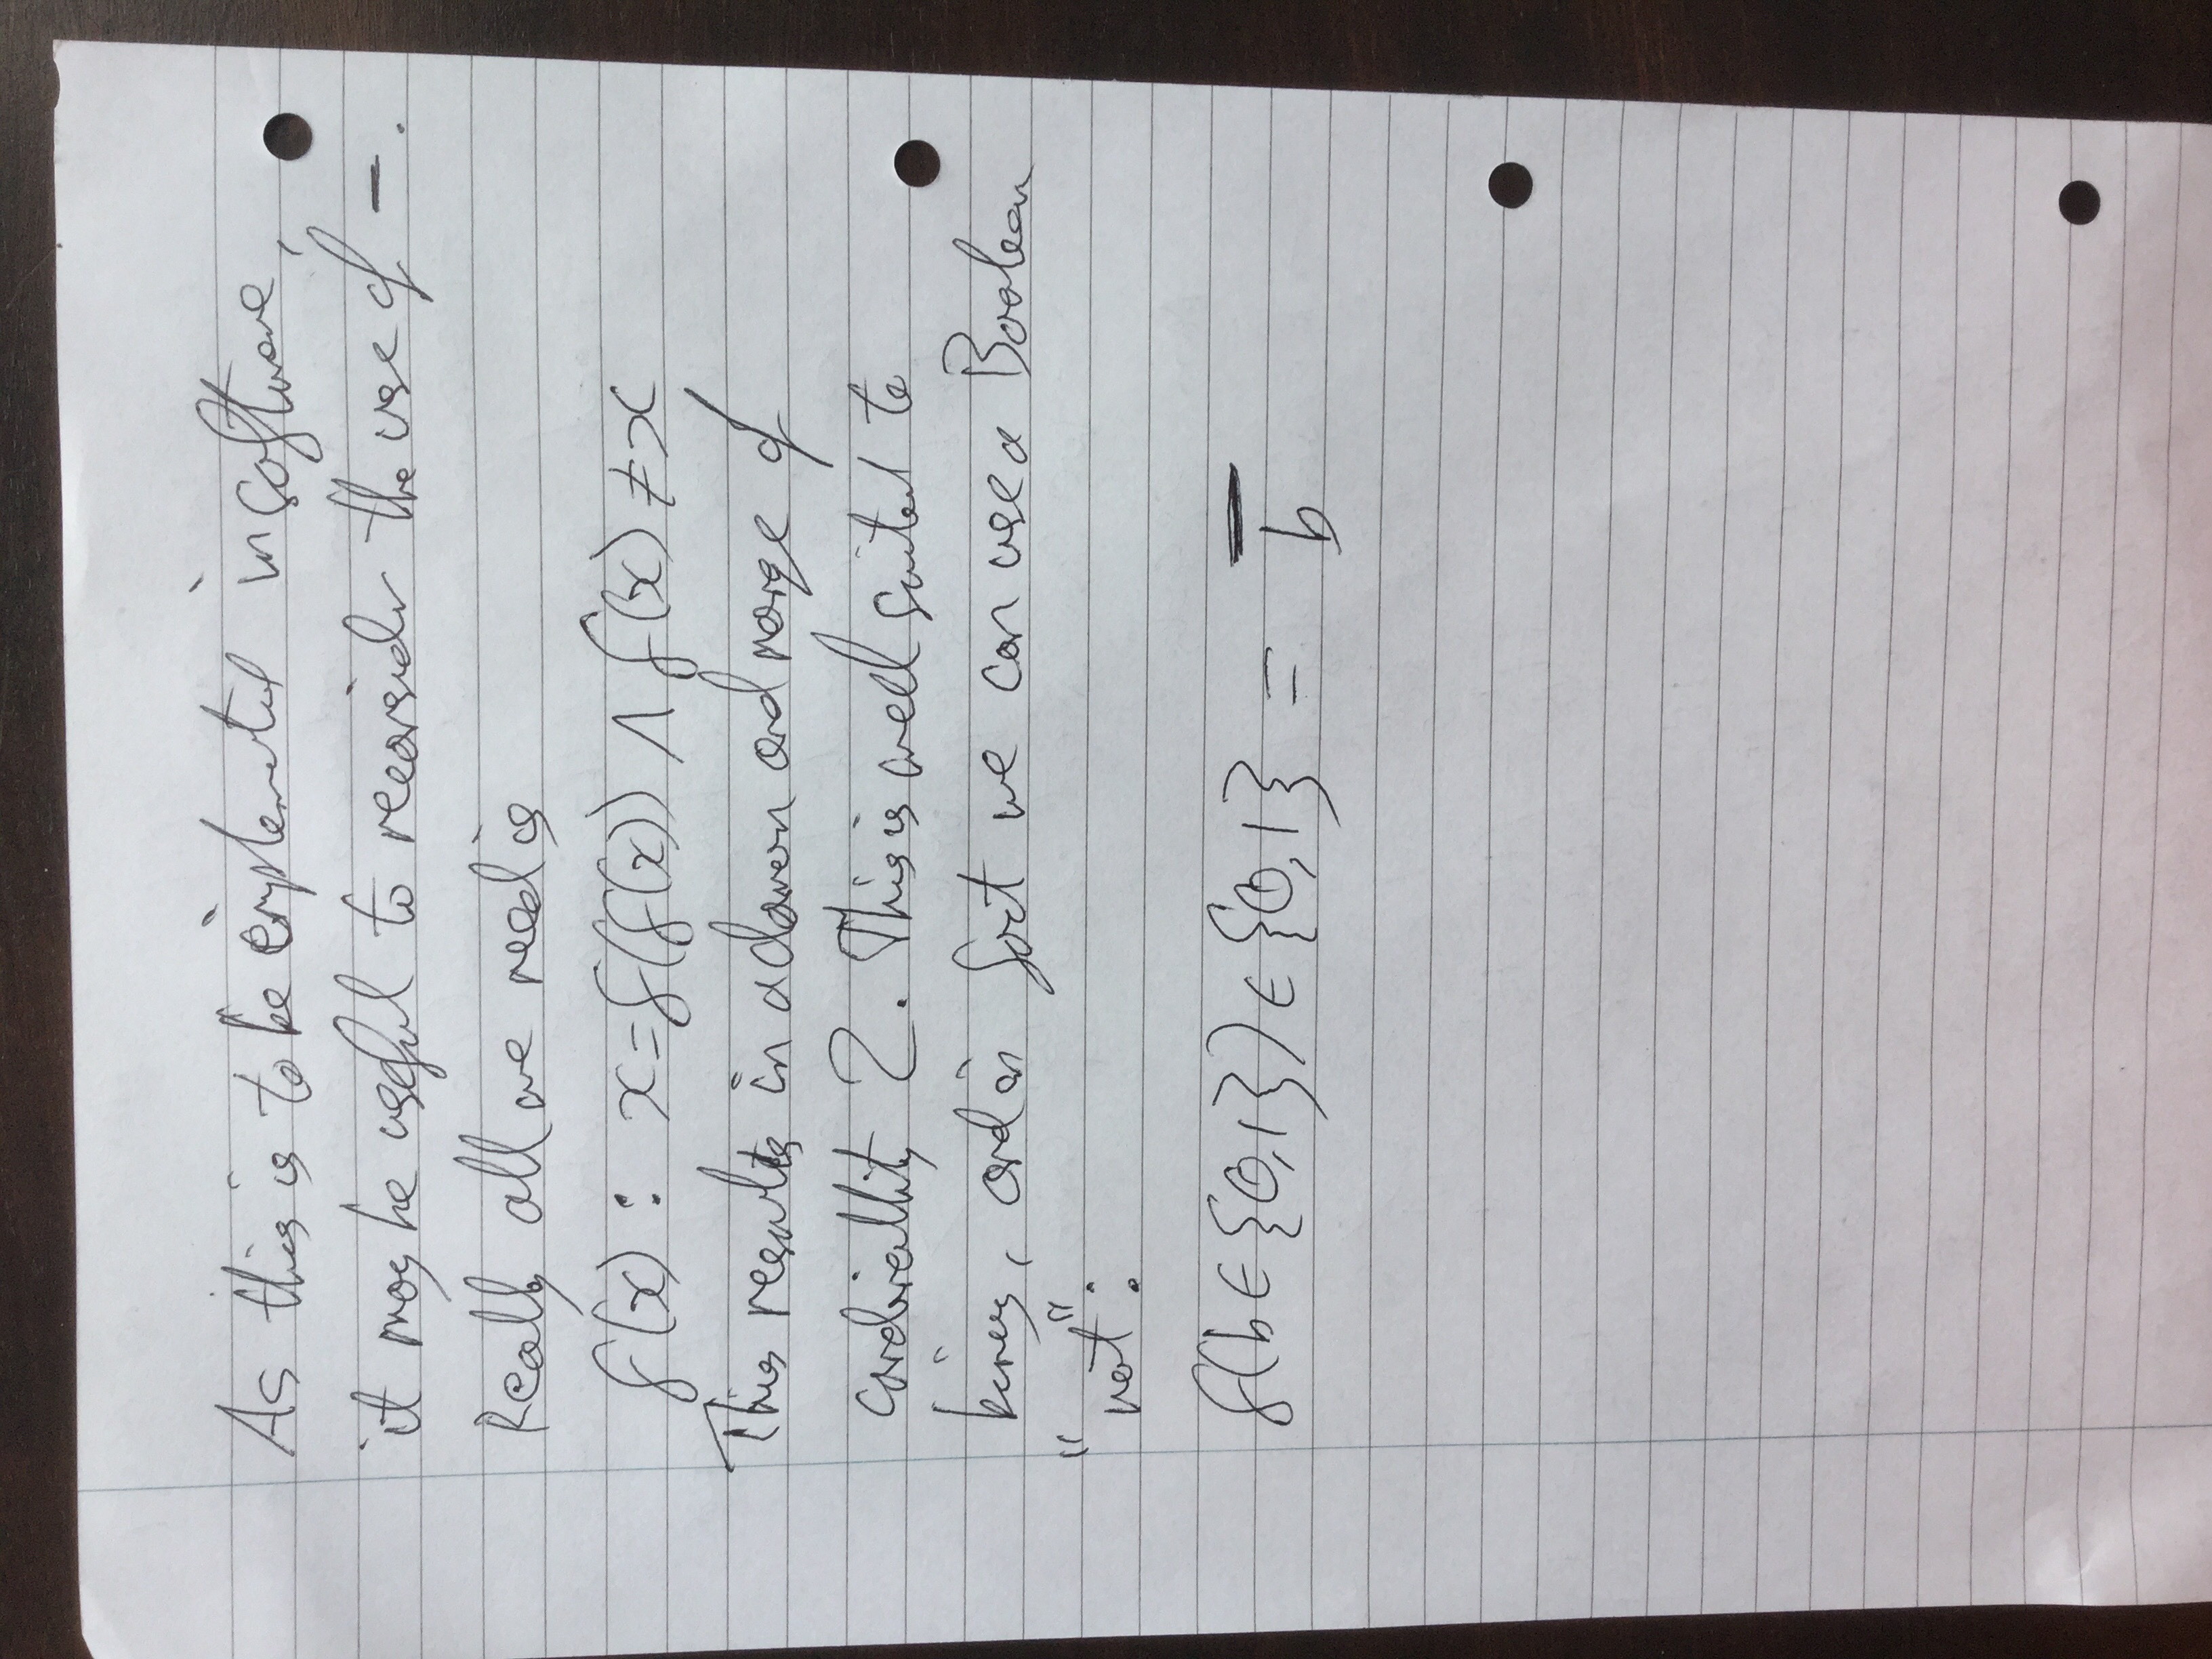
\includegraphics[height=0.3\textheight]{../psfiles/hadamard_2.eps}

\includegraphics[height=0.3\textheight]{../psfiles/hadamard_3.eps}

\includegraphics[height=0.3\textheight]{../psfiles/hadamard_4.eps}
\includegraphics[height=0.3\textheight]{../psfiles/hadamard_5.eps}
\end{center}
\caption{Visualisations of ``$2^n$'' Hadamard matrices}\label{fig:hadvis}
\end{figure}

    \subsection{Implementation}

\begin{longlisting}
\inputminted{python}{../src/hadamard_matrix.py}
\caption{Hadamard matrix generation}\label{lst:hadgen}
\end{longlisting}

    \section{Unit tests}

    For all the core programs, I have also written unit tests. These aim to
    verify that the program works by presenting a number of test cases, and
    seeing if the program produces the correct output. These both help to ensure
    correct behaviour, and can serve as a more practical reference of how I
    expect functions to behave.

\begin{longlisting}
\inputminted{python}{../src/test_encode_hamming.py}
\caption{Unit tests for encode\_hamming}\label{lst:testhammingbin}
\end{longlisting}

\begin{longlisting}
\inputminted{python}{../src/test_hadamard_matrix.py}
\caption{Unit tests for hadamard\_matrix}\label{lst:testhadamardmat}
\end{longlisting}

    \section{Miscellaneous listings}

    Below are all the listings that I don't consider to be important to the
    DNA barcoding part of my dissertation, but have still included as it is
    material that I have produced for my EP, and illustrate some of the work
    that has gone into the production of the actual dissertation.

\begin{longlisting}
\begin{minted}{python}
for p_ind in (1 << pwr for pwr in range(5)):
    print(r"    {} \\".format(" & ".join(str(i) for i in range(1, 33) if i & p_ind)))
\end{minted}
\caption{Generating Hamming coverage indices}\label{lst:hamtab}
\end{longlisting}

\begin{longlisting}
\begin{minted}{python}
def add_color(s, ind):
    return r"{}\textcolor{{blue}}{{{}}}{}".format(s[:ind], s[ind], s[ind+1:])

table = zip(*[[i for i in range(1, 33) if i & p_ind] for p_ind in (1 << pwr for pwr in range(5))])
print("\n".join(r"    {} \\".format(" & ".join(r"\texttt{{{}}}".format(add_color(bin(i)[2:].rjust(5, "0"), 4 -sig_ind))
            for sig_ind, i in enumerate(row)))
            for row in table))
\end{minted}
\caption{Generating binary table}\label{lst:hamcol}
\end{longlisting}

\begin{longlisting}
\inputminted{postscript}{../psfiles/hamming_visualisation.ps}
\caption{Hamming index coverage}\label{lst:hamps}
\end{longlisting}

\begin{longlisting}
\inputminted{python}{../src/generate_ham_vis.py}
\caption{Hadamard visualisation (uses code in \ref{lst:hadps})}\label{lst:hadpy}
\end{longlisting}

\begin{longlisting}
\inputminted{postscript}{../src/hadamard_template.ps}
\caption{Template for Hadamard graphic}\label{lst:hadps}
\end{longlisting}

    \section{Source}

    This document consists of about
    \input{|"texcount dissertation.tex | awk '/^Words in text/{print $NF-1}'"}
    words.

    All code and source \TeX/\LaTeX{} files can be found at
    \url{https://github.com/elterminad0r/EPQ}.

    Unless stated otherwise, all work has been produced by me, including
    graphics, and source code.

%TODO classifications of codes by number of correctable errors

\nocite{*}

\bibliographystyle{agsm}
\bibliography{sources}
\end{document}
